\chapter{Introduction}
\section{Context}
\subsection{3D viewers}
-> Applications?

-> Who uses them?

-> What for?

\subsection{\acs{bim} geometry} \label{subsec:bimGeometry}
% -> What is \ac{bim}? (short)

% -> Extend of \ac{bim} geometry?
% -> Complexity of \ac{bim} geometry?
The 3D model of a building consists of a multitude of sub-models, describing objects for all the different stakeholders participating in the project. Some describe very large objects, and some very small parts. Both can be defined in their most simple and abstract form or have an intricate and complex geometry. As a basic example, can a door simply be defined as a box, or up to the level of the screw-thread for the hinge system. The level of abstraction is here described as the \ac{lod}, it is most of the time pre-selected for the needs of a \ac{bim} model, and is applied throughout a single model.

\begin{figure}[h]
    \centering
    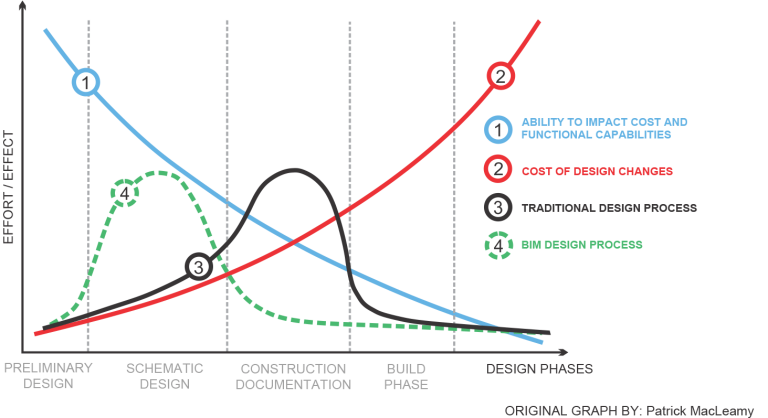
\includegraphics[width=0.5\textwidth]{figures/BIM grafiek.png}
    \caption{Evolution of \acs{lod} during the life-cycle of a building.}
    \label{fig:bimGraph}
\end{figure}

As shown in Figure~\ref{fig:bimGraph}, a standard BIM workflow goes through multiple phases each with their associated model and \ac{lod}. The \ac{lod} is a very important concept in the \ac{aec} industry, as it allows for a very efficient workflow. Approaching the modelling step from a top-down perspective, starting with rougher geometries describing the rougher ideas of a concept model and evoluting to a more refined model for the construction phase. As last and longest standing model, can a higher \ac{lod} be used to describe subtle changes in the evolution of a building.

This amount of data, both accounting for the \\
-> Some data BB models

\subsection{\acs{ldbim}}
% -> ! Focus on geometry

% -> What is \ac{ldbim}?

% -> Why the need / What are the advantages of \ac{ldbim}?

% -> Context od enrichment and complexity

% -> Own definition of \ac{ldbim}

The interconnectivity of semantics can also be applied to geometry descriptions. Which could allow the co-existence of multiple \ac{lod}s in a single model. Besides storing the evolution of a single element's geometry, it allows the linking of the different \ac{lod}s to each other. In contrary to standard \ac{bim} models, as explained in \ref{subsec:bimGeometry}.

\subsection{Computing power dilemma} \label{subsec:computingPower}
The enrichment of the \ac{ldbim}-graph also comes with a cost. The amount of data that needs to be stored and processed is much larger than a standard \ac{bim} model. Viewers greatly suffer from enrichment as most standard applications require the full model to be loaded in memory.

% -> What is the hardware problem?
Although most office computers used in the \ac{aec} industry are powerful enough to handle large models, the hardware used in the field is not. The most common hardware used in the field is a tablet or a laptop. Both of these are not powerful enough to handle the amount of data required to display a \ac{ldbim} model. This is a problem as these low-power devices are the only solution when it comes to mobility. Furthermore, the size of the models that are more and more enriched can, in some cases, pose a problem to the hardware of a standard office computer.
% -> Why is it that important for the \ac{aec} industry?


\section{Research questions}
% -> Why the need for this thesis? (why a \ac{ldbim} viewer?)
% -> What is the possible solution? (Culling algorithms)
% -> Why the need for research questions?
% (culling algorithms are not new, always progress, see later)-
It can be inferred from \ref{subsec:computingPower} that filtering is necessary in order to visualize the geometry of a \ac{ldbim} model, due to its complexity and size. This filtering step, as shown in Figure~\ref{fig:firstIdea}, is also known as culling in 3D computer graphics. Culling is the process of removing objects, or parts of objects, from the scene that are not visible to the user. This is done to reduce the amount of data that needs to be processed and stored. Implementing such technology in the context of \ac{ldbim} is the proposal of this thesis. The main goal being the introduction of similar algorithms within this context. As culling algorithms are not new and part of a field of research in continuous expansion.

The research questions are therefore focused on the feasibility of this introduction. And propose a set of possible solutions tailored to this specific problem, while highlighting possibilities for future research and specific use cases.

\begin{figure}[h]
    \centering
    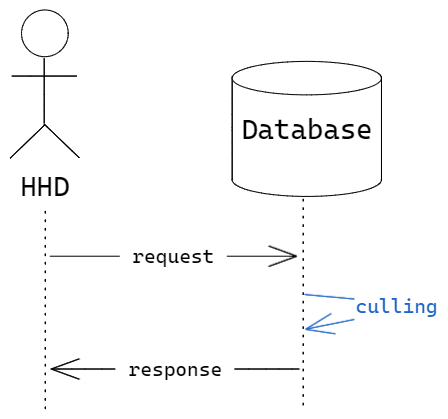
\includegraphics[width=0.4\textwidth]{figures/firstIdea.png}
    \caption{Basic principle}
    \label{fig:firstIdea}
\end{figure}
Figure~\ref{fig:firstIdea} illustrates the basic idea of this thesis. Being the extra step inside the communication between a user, here represented as a \ac{hhd}, and a database storing the model. A \ac{hhd} has been chosen to illustrate a low-powered device used in the field, that requires a lightweight 3D viewer to visualize and explore the digital twin of the building. The \ac{hhd} is assumed to have no knowledge of the \ac{ldbim} model, and only receives the geometry that is required to be displayed from the database. On the other hand, the database is assumed to have, or access to, all the knowledge of the model and the needed semantic to perform the culling.

\subsection[Can \acs{ldbim} be culled?]{To which extent can \acs{ldbim} geometry be culled \\
    to be streamed to lightweight viewers?}
% -> What can be culled exactly?
This thesis focuses on cumputing with data snippets or triples inside a \ac{ldbim} model, not wihtin. Meaning that the smallest unit of data that can be culled is the one described in one triple, in the most likely scenario: a single \ac{lod} of a single element. It implies that geometry is defined and separated at the object-level. It also implies that culling thechniques such as back-face culling will not be handled in this thesis, and will be left to the viewer itself, not the database.

% -> What needs to be streamed?
Which snippets of data are needed by the viewer? Is part of the question. The basic needs of the viewer consists firstly of the geometry itself, selecting the right geometry format for the application as well as the additional visual information such as color, texture, etc. Secondly, the identifier of each element is of crucial importance to maintain the link to other semantic ressources in the graph. Enabling the viewer to retrieve those ressources for a multitude of usecases. Transforming it into a user-friendly visual query tool.

% -> What is the impact of culling on the viewing experience?
The impact of the culling on the performance of the viewer will greatly determine the mutl

\subsection[Can existing semantic be used?]{Can existing semantic and ontologies be used\\
    to feed possible culling algorithms?}
-> What are ontologies?

% -> What are the advantages of using ontologies?
The 

% -> Can GIS ontologies be used too?


\section{Research objectives}
\subsection[Advantages of LDBIM]{Bring forward the advantages of \acs{ldbim} for visualization of big 3D models}
-> Showcase that existing models are already mature enough for these usecases.

->
\subsection[Showcase the feasibility]{Showcase the feasibility of \acs{ldbim} for visualization of big 3D models}
->